%
% Problem
\chapter{Problem Formulation} \label{chap::problem}


\section{Omni-wheeled robot} \label{sect::system}
The robot can be represented as a rigid body in a planar space. The location of the robot's \ac{COM} is defined as \lsymb{$\vec p_0\in\R^2$}{Location of the robot's center point} and the yaw of the robot is represeted as \gsymb{$\psi\in\R$}{Roll of the robot}.

Assuming the robot has \lsymb{$n\in\Z_{> 0}$}{Number of wheels} wheels, we can define their 


\section{Dynamic Model}

\newpage
\subsection{Motor Dynamics Identification}

The motors in our robot are controlled by velocity inputs. We will represent the inputs of the i-th motor as \lsymb{$u_i\in[-1,1]$}{i-th motor input}. The motors are also equipped with encoders from which we can deduce the angle of each wheel, denoted as \gsymb{$theta_i\in\R$}{i-th wheel angle}.

We can try to identify the model using process model identification. A tool that, given some identification data and a transfer function with unknown parameters, estimates the value of the parameters. We will assume that the relationship between input velocity and the real velocity follow a linear transfer function:
\begin{equation}
\frac{\dot{\theta_i}(s)}{u_i(s)}=\frac{K_i}{1+\tau_i s}
\rightarrow
\frac{\theta_i(s)}{u_i(s)}=\frac{K_i}{s(1+\tau_i s)}
\end{equation}

Which corresponds to the following set of ODEs:
\begin{equation}
\dot{\theta_i}+\tau\ddot{\theta_i}=u\,K
\end{equation}

To obtain the identification data we can make the arduino generate a square wave and record the data from the encoder. This will give us data discretized with different time-intervals as the time-interval will depend on the loop size. To get data with equal time-intervals we can set a higher sampling frequency and interpolate the values between each sample.

When identifying the model we saw that the values of $K$ were different for varying amplitudes as we can see in \cref{fig:K_u}.

\todo{Do experiments for higher values of amplitude (when lab is empty)}
\begin{figure}[h]
	\centering
	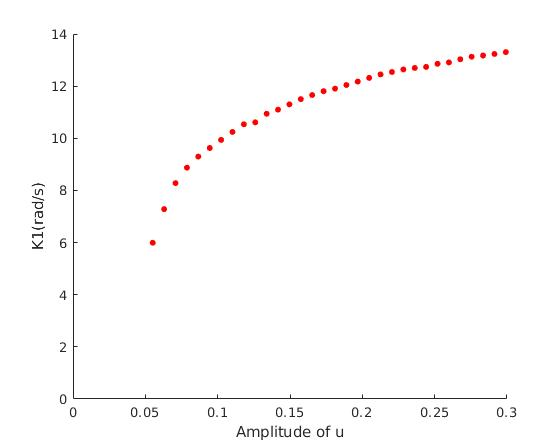
\includegraphics[width=0.31415\textwidth]{Figures/K_u}
	\caption{Relationship between $K_1$ and the amplitude of $u$}
	\label{fig:K_u}
\end{figure}


As the relationship looks like it has a vertical and a horizontal asymptote, we will try to model it with a rational function of the form:
\begin{equation}
K_i=\frac{a_i\,u_i+b_i}{u_i+c_i}
\end{equation}

\begin{figure}[h]
	\centering
	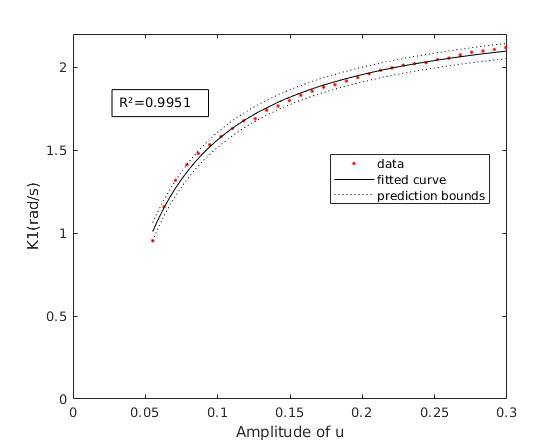
\includegraphics[width=0.31415\textwidth]{Figures/K_u_pred}
	\caption{Predicted relationship between $K_1$ and the amplitude of $u$}
	\label{fig:K_u_pred}
\end{figure}
\todo{see if $\tau$ depends on u}






\subsection{Aerodynamic Drag}
We will use the same model for aerodynamic drag model as in \cite{Potdar2018}. The drag on the payload, denoted as \lsymb{$\vec F_{Dl}\in\R^3$}{Aerodynamic drag on the payload}, is modeled using a quadratic drag model, while the drag on each quadrotor, denoted as \lsymb{$\vec F_{Di}\in\R^3$}{Aerodynamic drag on the $i$-th drone}, is modeled using a linear drag model.
\begin{alignat}{2}
\vec F_{Dl} &= 
-k_{Dl}\|\dot{\vec p}_l\|^2\frac{\dot{\vec p}_l}{\|\dot{\vec p}_l\|} &&= 
-k_{Dl}\|\dot{\vec p}_l\|\dot{\vec p}_l
\label{eq::dragl}
\\
\vec F_{Di} &= 
-k_{Di}\|\dot{\vec p}_i\|\frac{\dot{\vec p}_i}{\|\dot{\vec p}_i\|} &&= 
-k_{Di}\dot{\vec p}_i \quad\foralli
\label{eq::dragi}
\end{alignat}

Where \lsymb{$k_{Dl}\in\R$}{Drag constant of the payload} and \lsymb{$k_{Di}\in\R$}{Drag constant of the $i$-th quadrotor} are the drag constants identified in \cite{Potdar2018}.

\subsubsection{Drag Inclusion in \ac{EOMs}}
To use include drag in our problem we need to include the drag force calculated in equations \ref{eq::dragl} and \ref{eq::dragi} in the \ac{EOMs} declared in equations \ref{eq::eom2} and \ref{eq::eom3}.

The drag force on the drones $\vec F_{Di}$ can be added to the input force $\vec F_{ui}$ (we will denote this sum as \lsymb{$\vec F_{uDi}$}{addition of $\vec F_{ui}$ and $\vec F_{Di}$}). The drag force on the payload can be included by subtracting $\frac{\vec F_{Dl}}{m_l}$ from all appearances of $\ddot{\vec p}_l$ in the \ac{EOMs}, in the same way that $g\vec e_3$ is subtracted. The resulting \ac{EOMs} from these changes are:


\begin{align}
\dot{\vec q}_i& = \vec w_i \times \vec q_i \quad \foralli \label{eq::eom_drag1}
\\
\vec M_q(\ddot{\vec p}_l-g \vec e_3-\frac{\vec F_{Dl}}{m_l}) &= \sum_{i=1}^{n}(-m_il_i\|\vec w_i\|^2\vec q_i +\vec F_{uDi}^\parallel) \label{eq::eom_drag2}
\\
\dot{\vec w}_i &=\frac{1}{l_i}\vec q_i\times(\ddot{\vec p}_l-g \vec e_3-\frac{\vec F_{Dl}}{m_l})-\frac{1}{m_il_i}(\vec q_i\times\vec F_{uDi}^\perp) \quad \foralli \label{eq::eom_drag3}
\end{align}

\subsection{Environment Definition}
The environment is defined as a 3 dimensional box with the origin in the floor's center. We denote the box's dimensions as \lsymb{$\vec{dim}\in\R^3_{>0}$}{Environment dimensions}. A schematic of the environment can be seen in \cref{fig::environment}.

\begin{figure}
	\centering
	\begin{tikzpicture}
	\pic at (1,-3) {annotated cuboid={width=250, height=200, depth=150, scale=.02, units=m}};
	\end{tikzpicture}
	\caption{Environment Schematic}
	\label{fig::environment}
\end{figure}


\subsection{Obstacle Modeling}
\label{subsect::obstacle_modeling}
Obstacles are modeled as three dimensional boxes and their behavior is modeled as linear movement using a Kalman Filter. This is required so that the planner takes into account future movement of the obstacles. The number of obstacles is denoted by \lsymb{$n_{obs}\in\Z_{\ge0}$}{Number of obstacles}, their center position by \lsymb{$\vec{p}_{obs_i}\in\R^3$}{Position of the $i$-th obstacle} and their dimension by \lsymb{$\vec{dim}_{obs_i}\in\R^3_{>0}$}{Dimension of the $i$-th obstacle}. 

Often we will use the smallest ellipsoid that contains the box.  The equations to find the radial dimensions of the ellipsoid (denoted as \lsymb{$\vec{dim}_{ell_i}\in\R^3$}{Ellipsoid dimensions of the $i$-th obstacle}) are:

\begin{figure}
\usetikzlibrary{decorations.pathreplacing}
\centering
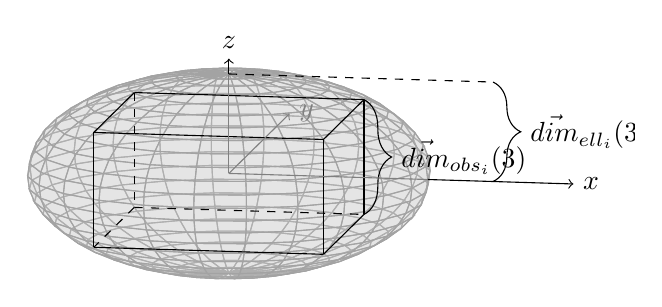
\begin{tikzpicture}
\begin{axis}[%
width=0.8\textwidth,
axis equal,
view={10}{10},
axis lines = none,
xmax=3,
ymax=3,
zmax=1,
ticks=none,
colormap={}{ gray(0cm)=(0.8); gray(1cm)=(0.8);}
]
\addplot3[%
fill opacity=0.3,
surf,
domain=0:2*pi,y domain=0:pi,
z buffer=sort
]
({sqrt(3)*1*cos(deg(x))*sin(deg(y))}, {sqrt(3)*1 *sin(deg(x))*sin(deg(y))}, {sqrt(3)*.5*cos(deg(y))});
\draw (-1,1,.5)--(1,1,.5);
\draw (-1,-1,.5)--(1,-1,.5);
\draw[dashed] (-1,1,-.5)--(1,1,-.5);
\draw (-1,-1,-.5)--(1,-1,-.5);

\draw (1,1,.5)--(1,-1,.5);
\draw (-1,1,.5)--(-1,-1,.5);
\draw (1,1,-.5)--(1,-1,-.5);
\draw[dashed] (-1,1,-.5)--(-1,-1,-.5);

\draw (1,1,.5)--(1,1,-.5);
\draw[dashed] (-1,1,.5)--(-1,1,-.5);
\draw (1,-1,.5)--(1,-1,-.5);
\draw (-1,-1,.5)--(-1,-1,-.5);

\draw[decorate,decoration={brace,amplitude=10pt,mirror}] (1,1,-.5)--(1,1,.5) node[midway,anchor=west,xshift=10pt]{$\vec{dim}_{obs_i}(3)$};
%\node[anchor=west] at (1.1,1,0) {$\vec{dim}_{obs_i}(3)$};
\draw[dashed] (0,0,.866)--(2.3,0,.866);
\draw[decorate,decoration={brace,amplitude=10pt}] (2.3,0,.866)--(2.3,0,0) node[midway,anchor=west,xshift=10pt]{$\vec{dim}_{ell_i}(3)$};


\draw[color=gray] (0,0,0)--(1.732,0,0);
\draw[->] (1.732,0,0)--(3,0,0) node[anchor=west]{$x$};

\draw[->,color=gray] (0,0,0)--(0,3,0) node[anchor=west]{$y$};


\draw[color=gray] (0,0,0)--(0,0,.866);
\draw[->] (0,0,.866)--(0,0,1) node[anchor=south]{$z$};
\end{axis}
%
\end{tikzpicture}
\caption{Obstacle dimensions}
\label{fig::obstacle_dimensions}

\end{figure}

\begin{equation}
\vec{dim}_{ell_i} = \frac{\sqrt{3}}{2}\vec{dim}_{obs_i}
\quad\foralli[obs]
\end{equation}

A schematic of an obstacle and its dimensions can be seen in \cref{fig::obstacle_dimensions}. For further explanation refer to his thesis\cite{Potdar2018}.